\documentclass[preprint,12pt,TurnOnLineNumbers]{JASAnew}

\usepackage{color,soul}

\pdfoutput=1
\hyphenation{echo-sounders}
\renewcommand{\figurename}{Figure}

\newcommand{\ek}{Simrad EK80}

\newcommand{\timesym}{t}
\newcommand{\freqsym}{f}
\newcommand{\samplesymt}{n}
\newcommand{\samplesymf}{m}
\newcommand{\genidxsym}{i}

\newcommand{\channelsym}{u}
\newcommand{\nchannels}{N_{\textrm{u}}}

\newcommand{\stagesym}{v}
\newcommand{\nstages}{N_{\textrm{v}}}

\newcommand{\fs}{f_{\textrm{s}}}
\newcommand{\fsdec}{f_{\textrm{s,dec}}}
\newcommand{\fstart}{f_{\textrm{start}}}
\newcommand{\fstop}{f_{\textrm{stop}}}
\newcommand{\fc}{f_{\textrm{c}}}
\newcommand{\fn}{f_{\textrm{n}}}


\newcommand{\zrxe}{z_{\textrm{rx,e}}}
\newcommand{\ztde}{z_{\textrm{td,e}}}

\newcommand{\ptxe}{p_{\textrm{tx,e}}}
\newcommand{\prxe}{p_{\textrm{rx,e}}}

\newcommand{\ntd}{n_{\textrm{td}}}
\newcommand{\tnom}{\tau}
\newcommand{\teff}{\tau_{\textrm{eff}}}


\newcommand{\ytxe}{y_{\textrm{tx,e}}}
\newcommand{\ytxa}{y_{\textrm{tx,a}}}
\newcommand{\yrxa}{y_{\textrm{rx,a}}}
\newcommand{\yrxe}{y_{\textrm{rx,e}}}

\newcommand{\ytx}{y_{\textrm{tx}}}
\newcommand{\ytxnorm}{\tilde{y}_{\textrm{tx}}}
\newcommand{\ytxfd}{y_{\textrm{tx,f,d}}}
\newcommand{\yrx}{y_{\textrm{rx}}}
\newcommand{\yrxorg}{y_{\textrm{rx,org}}}
\newcommand{\ymf}{y_{\textrm{mf}}}

\newcommand{\ytd}{y_{\textrm{td}}}

\newcommand{\ypc}{y_{\textrm{pc}}}
\newcommand{\ypctarget}{y_{\textrm{pc,t}}}
\newcommand{\ypcspread}{y_{\textrm{pc,s}}}
\newcommand{\ymfauto}{y_{\textrm{mf,auto}}}
\newcommand{\ymfautored}{y_{\textrm{mf,auto,red}}}

\newcommand{\ptxauto}{p_{\textrm{tx,auto}}}

\newcommand{\ypctargetf}{Y_{\textrm{pc,t}}}
\newcommand{\ypctargetnormf}{\tilde{Y}_{\textrm{pc,t}}}
\newcommand{\ypcvolumef}{Y_{\textrm{pc,v}}}
\newcommand{\ypcvolumenormf}{\tilde{Y}_{\textrm{pc,v}}}

\newcommand{\ymfautof}{Y_{\textrm{mf,auto}}}
\newcommand{\ymfautoredf}{Y_{\textrm{mf,auto,red}}}

\newcommand{\prxetf}{P_{\textrm{rx,e,t}}}
\newcommand{\prxevf}{P_{\textrm{rx,e,v}}}


\newcommand{\fstage}{k}
\newcommand{\decfac}{D}
\newcommand{\lfl}{L_{\textrm{fl}}}
\newcommand{\hfl}{h_{\textrm{fl}}}
\newcommand{\hannw}{w}
\newcommand{\hannwnorm}{\tilde{\hannw}}
\newcommand{\nw}{N_{\hannw}}
\newcommand{\hannwpart}{\gamma}
\newcommand{\tslide}{t_w} 

\newcommand{\bs}{\sigma_{\textrm{bs}}}
\newcommand{\mysp}{S_p}
\newcommand{\ts}{\textrm{TS}}
\newcommand{\sv}{S_{\textrm{v}}}

\newcommand{\range}{r}
\newcommand{\rangeref}{r_0}
\newcommand{\athw}{\phi}
\newcommand{\along}{\theta}
\newcommand{\gain}{g}
\newcommand{\gainzero}{g_0}
\newcommand{\eqang}{\psi}

\newcommand{\rtarget}{r_{\textrm{target}}}
\newcommand{\alongtarget}{\theta_{\textrm{target}}}
\newcommand{\athwtarget}{\phi_{\textrm{target}}}


\newcommand{\wlen}{\lambda}
\newcommand{\cw}{c}
\newcommand{\absorp}{\alpha}

\newcommand{\dft}{\textrm{DFT}}
\newcommand{\ndft}{{N_{\textrm{DFT}}}}
\newcommand{\ndftw}{_{\nw}}
\newcommand{\atan}{\textrm{arctan2}}
\newcommand{\anglefalong}{\gamma_\along}
\newcommand{\anglefathw}{\gamma_\athw}

\newcommand{\sigmabs}{\sigma_{\textrm{bs}}}

\begin{document}

\title[]{Quantitative processing of broadband data as implemented in a scientific splitbeam echosounder}

\author{Lars Nonboe Andersen}
\email{lars.nonboe.andersen@kongsberg.com}
\affiliation{Kongsberg Maritime AS, Strandpromenaden 50, 3191, Horten, Norway}

\author{Dezhang Chu}
\affiliation{Fishery Resource Analysis and Monitoring Division, Northwest Fisheries Science Center, National Marine Fisheries Service, National Oceanic and Atmospheric Administration, 2725 Montlake Blvd. E. Seattle, WA, 98112, USA}

\author{Nils Olav Handegard}
\affiliation{Marine Ecosystem Acoustics, Institute of Marine Research, Bergen, 5001, Norway}

\author{Harald Heimvoll}
\affiliation{Kongsberg Maritime AS, Strandpromenaden 50, 3191, Horten, Norway}

\author{Rolf Korneliussen}
\author{Gavin J. Macaulay}
\author{Egil Ona}
\affiliation{Marine Ecosystem Acoustics, Institute of Marine Research, Bergen, 5001, Norway}

\author{Ruben Patel}
\affiliation{Codelab, Bergen, Norway}

\author{Geir Pedersen}
\affiliation{Marine Ecosystem Acoustics, Institute of Marine Research, Bergen, 5001, Norway}

\begin{abstract}
The use of quantitative broadband echosounders for biological studies and surveys offers considerable advantages over narrowband echosounders. These include improved spectral-based target identification and significantly increased ability to resolve individual targets. Biological studies and surveys typically require accurate measures of backscatter strength and we present here a systematic and comprehensive explanation of how to derive quantitative estimates of target strength and volume backscattering, as a function of frequency from broadband echosounder signals.

\end{abstract}

\maketitle


\section{Introduction}

Active acoustics is an efficient method for remote sensing of marine ecosystems. These methods have been used to cover a wide range of spatial and temporal scales, ranging from tens of km \citep{makris_fish_2006} to small scale behaviour patterns \citep{klevjer_split-beam_2003}, and can provide information on key forage species, including fish and zooplankton, linking primary producers and top predators as well as other taxonomic groups important for the ecosystem functioning \citep{benoit-bird_ecological_2016}. As early as 1935, Oscars Sund observed the distribution of spawning cod in the Lofoten area using a single beam echosounder \citep{sund_echo_1935}. The method was further developed to map the abundance of fish, driven by the need for fisheries management \citep{Simmonds2005Fisheries}. More recently, the methods have been deployed on a wide range of platforms, including observatories, autonomous underwater vehicles \citep{fernandes_autonomous_2003}, uncrewed surface vehicles \citep{de_robertis_uncrewed_2021} and vessels of opportunity, observing a wide range of ecosystem processes across different spatial and temporal scales \citep{godo_marine_2014}.

Several different configurations of acoustic instruments are available, including multibeam sonars \citep{gerlotto_two_1999}, synthetic aperture sonar, omnidirectional sonars \citep{misund_improved_1996}, acoustic imaging sonars \citep{jaffe_ftv_1995} as well as single- and multibeam echosounders \citep{trenkel_new_2008}. Narrowband single beam echosounders have been used extensively in fisheries management and ecosystem monitoring, and methodology for using these systems are well developed. The ability for accurate calibration of the system has made these especially useful for providing data for fisheries management \citep{Simmonds2005Fisheries}.

Recent commercially available single beam echosounders produce pulses with a wide and continuous frequency range (broadband pulses), as opposed to conventional single frequency systems. This provides significantly better along-beam resolution, a higher signal to noise ratio than narrowband pulses \citep{Chu1998Application, ehrenbergFMSlideChirp2000}, and  improved frequency resolution for backscatter categorization \citep{korneliussen2018}.

Broad banded echosounders have been pursued actively for ecology in particularly based on the promise of improved categorization of species or group of species. Using high frequency broadband acoustics (150-600 kHz) Lavery et al \citep{lavery_measurements_2010} showed that broadband helped reduce the ambiguities in interpretation of acoustic scattering from zooplankton and oceanic microstructure. \citep{Stanton2012Resonance} used low frequency broadband pulses (1-6 kHz) with frequency content covering the resonance of swimbladdered fish, demonstrating both the spectral resolution and ability to classify size classes of fish within fish assemblages. \citep{blanluet_characterization_2019} used broadband, with ground truthing, to identify that the composition of two Sound Scattering Layers (SSL) detected in the Bay of Biscay in springtime was characterized and identifying fine scale heterogeneity within the SSLs. While unsuccessful in discriminating between several species of fishes with large  swimbladders during the Alaska pollock survey, \citep{bassett_broadband_2018} showed that broadband may be helpful in characterizing smaller fishes with swimbladder and euphausiids. \citep{benoit-bird_exploring_2020} was able to effectively discriminate three monospecific aggregations of species (hake, anchovy and krill) using broadband data (45-170 kHz), while attempts to classify using narrowband multifrequency failed.

The increased spatial resolution is another aspect of broadband acoustics that are actively being used both for improved categorization and increased ability to resolve targets near each other or near boundaries such as the seafloor. \citep{lavery2017} explored different broadband pulse shapes to increase successful resolution of single targets in proximity as well as near boundaries in tank experiments. By applying high frequency broadband pulses to fish-like artificial targets, \citep{kubilius_remote_2020} demonstrated the potential for acoustic sizing of individually resolved fishes in a controlled ex situ environment. Utilizing the increased spatial resolution \citep{hasegawa_situ_2021} were able to isolate single fishes and discriminate successfully between average frequency responses of walleye pollock and pointhead flounder.

An equally interesting outcome from the increased resolution and broad frequency bands is the ability to infer behavioural information on both single individuals, groups of individuals, and interaction between individuals or groups. \citep{Traykovski1998Effect} was able to extract orientation information about krill from using a combination of high frequency broadband acoustics and acoustic modelling. Fine-scale observations of single targets facilitated the study of interactions between prey and predators, capelin and cod, in the Barents sea (\citep{skaret_diel_2020}).

There have been several scientific broadband echosounder systems developed for laboratory use \citep{Conti2003Wide-bandwidth, Forland2014Scattering, chu1992}, some prototype or custom-made systems \citep{Zakharia1989Wide-band, Zakharia1996Wideband, Simmonds1996Species, Foote2005Measuring, Imaizumi2009Detection, Briseno-Avena2015ZOOPS, Barr2002Target} and some commercially available systems \citep{Gordon1998FishMASS, Zedel2003Acoustic, Stanton2010New, ehrenbergFMSlideChirp2000, dennyBroadbandAcousticFish1998}.

The theoretical foundation for signal processing comes from radar applications and is earlier documented for broadband echosounders \citep{stanton2008}. To tap the full potential of broadband echosounder data, further data processing methods are being developed \citep{lavery2017,bassett_broadband_2018}. Examples include adapting pulses to improve target separation as well as further parameters from the individual targets. Different send pulses can be envisioned as well as various methods for acoustic target classification. When translating equations into code, several choices must be made. Some of these are well founded in signal processing literature whereas others are of a more practical and ad-hoc nature. The latter is typically missing in conventional papers, and this makes it difficult to test the implementation of the signal processing methods in new echo sounders and post processing software.

The objective of this paper and associated code is to present a systematic and comprehensive description of the data processing steps for calibrated broadband echosounder data. The steps include pulse compression, target strength as a function of frequency [TS(f)], and volume backscattering strength as a function of frequency [Sv(f)]. The intention is that the code will be used to validate implementations in various echosounders and post processing software, provide a starting point for further developing signal processing, and serve as a learning resource for broadbanded acoustic data processing. We also note that the processing equations and methodology presented in this paper are similar to version 1.12.4 and earlier of the Simrad EK80 software. 

\section{Signal flow and initial processing}

\subsection{Accompanying code}
The code accompanying this paper is written in Python and is available as supplementary materials. All processing steps with respective figures in the paper can be reproduced by running main script (Main.py). Without loss of generality, we use the Simrad EK80 as an example since it is currently the most used broadband echosounder in the marine ecosystem acoustics field. By presenting the design goals, implementation details, and recommended procedures and processing required to obtain quantitative broadband data, the authors hope to encourage and facilitate the realistic use of broadband signals in marine ecosystem acoustics.

Our presentation uses nomenclature and approaches that are commonly used for narrowband echosounder systems, which were derived from radar processing \citep{cook1967}. In particular, the expressions for target strength ($\ts$) and volume backscattering strength ($\sv$) \citep{MacLennan2002consistent} are presented in a similar manner for broadband signals as for narrowband signals.

\subsection{System overview}
A basic echosounder system consists of a transducer, a transceiver, and a computer program that controls the operation of the transceiver and records received signals. During transmission the program defines the signals which are created as electric signals in the transceiver, converted to acoustic signals by the transducer and transmitted into the water. The acoustic signals propagate through the water, are reflected or scattered by objects in the water, and propagate back to the transducer. During reception the transducer converts the received acoustic signals to electric signals, which are received, pre-amplified, filtered, digitized, and processed in the transceiver, and then transferred to the controlling program for further data processing and storage (Fig. \ref{fi:ek_sys}). Many types of transmit signals are feasible - this paper considers only the transmission of linear frequency modulated signals (also known as linear chirps).

\begin{figure}
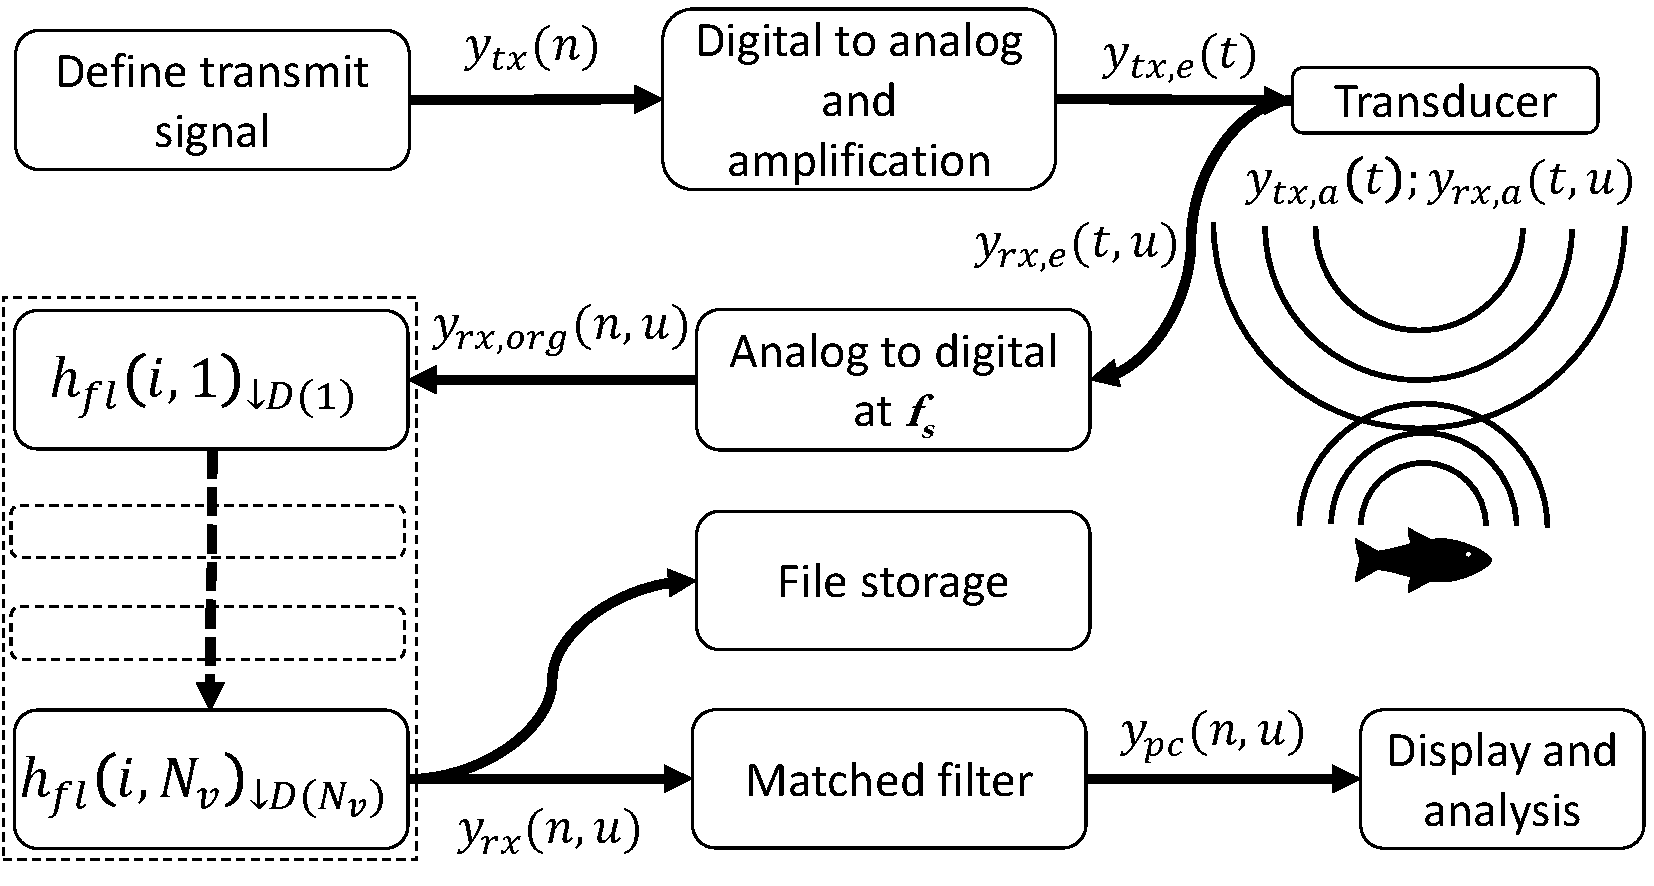
\includegraphics[width=16cm]{Fig_ek_sys}
\caption{\label{fi:ek_sys}Signal and data flow in the \ek{} system. An echosounder ping starts with the definition of a transmit signal (upper left) and ends with file storage (lower middle) and display and analysis (lower right). Note that all signals are complex-valued time-series.}
\end{figure}

\subsection{Signal generation}

The controlling computer program generates a short-duration digital transmit signal (a ping), $\ytx(\samplesymt)$, where $\samplesymt$ is a sample index in the discrete time domain. Typical BB pulses are linear upsweep pulses windowed by an envelope function. The generated signal $\ytxe(\timesym)$ is converted to an analogue electric signal and amplified by the transceiver to obtain analogue signal $\ytxe(\timesym)$. The analogue and amplified signal is passed on to the transducer to generate the transmitted acoustic signal $\ytxa(\timesym)$ in the water column, where $\timesym$ is the time for the (analog) signal. For a split-aperture echosounder system, there are typically three or four channels to allow estimation of the angle of arriving echoes, and the signal is typically transmitted with equal power across the channels.

In the example a linear sweep enveloped by a Hann function is implemented (Fig.~\ref{fi:ytx}). This is found in the class \verb|Calculation.generateIdealWindowedTransmitSignal|, where the parameters are the initial frequency, the final frequency, the pulse duration, the sampling rate, and the proportion of the signal that is tapered in each end, respectively. A tapering of 0 and .5 indicates no tapering and tapering across the whole signal, respectively.
\begin{figure}
\includegraphics[width=16cm]{Fig_ytx}
\caption{\label{fi:ytx} Ideal and enveloped transmit pulse between 34 kHz to 45 kHz with a slope of 0.057, as implemented in the EK80. The orange curve illustrate the effect of setting the slope to 0.5.}
\end{figure}

\subsection{Signal reception}

The returning acoustic signal, $\yrxa(\timesym)$, is received by each transducer sector, $\channelsym$, and converted to an analog electric signal, $\yrxe(\timesym,\channelsym)$, in the transducer and received by corresponding receiver channels, $\channelsym$, in the transceiver. The received electric signal, $\yrxe(\timesym,\channelsym)$, from each channel, $\channelsym$, is pre-amplified, filtered by an analog anti-aliasing filter, and digitized in the transceiver at a frequency of $\fs$, creating the digital signal, $\yrxorg(\samplesymt,\channelsym)$.

To remove noise and reduce the quantity of data, the sampled signal from each channel is filtered and decimated in multiple stages, $\stagesym$, using complex bandpass filters, $\hfl(\genidxsym,\stagesym)$, and decimation factors, $\decfac(\stagesym)$. The individual filter coefficients for each filter and decimation stage are indexed by $i$. The output signal from each channel, $\channelsym$, from each filter and decimation stage, $\stagesym$, is then given by:
%
\begin{equation}
\label{eq:yrx}
\yrx(\samplesymt,\channelsym,\stagesym) = \left( \yrx(\samplesymt,\channelsym,\stagesym-1) * \hfl(\genidxsym,\stagesym) \right)_{\downarrow \decfac(\stagesym)}, 
\stagesym = 1,\ldots,\nstages,
\end{equation}
%
where $\yrx(\samplesymt,\channelsym,0)$ is set to $\yrxorg(\samplesymt,\channelsym)$, being the signal before decimation, $*$ indicates convolution and $\nstages$ is the total number of filter stages. The output signal from the final filter and decimation stage, $\yrx(\samplesymt,\channelsym,\nstages)$, is shortened to $\yrx(\samplesymt,\channelsym)$ for convenience. For the output signal, $\yrx(\samplesymt,\channelsym)$, the decimated sampling rate, $\fsdec$, is given by:
%
\begin{equation}
\label{eq:fsdec}
\fsdec = \fs\prod_{\stagesym=1}^{\nstages} \frac{1}{\decfac(\stagesym)}.
\end{equation}
%
The characteristics of the bandpass filter and decimation factors are chosen with regard to the desired operating bandwidth, noise suppression levels, impulse response duration, and other common filter characteristics, with the aim of maintaining sufficient information in the data. In the example $N_v=2$. The frequency responses of the filters are shown in Figure~\ref{fi:fir}, and the corresponding filter coefficients and decimation factors are found in the test data set.

\begin{figure}
\includegraphics[width=16cm]{Fig_fir}
\caption{\label{fi:fir} The frequency (power) response of the filters in our test set.}
\end{figure}

The original sample data $\yrxorg(\samplesymt,\channelsym)$ are not available in the EK80 data files. Instead, the resulting filtered and decimated complex samples from each transducer channel $\yrx(\samplesymt,\channelsym)$ are stored in the data files. The data are recorded together with additional data such as from position and motion sensors and system configuration data in raw data files for display and analysis by processing software. The filter parameters are in this paper used to generate the transmit pulse for the matched filter, see below.


\subsection{Pulse compression}
To increase signal-to-noise ratio and resolution along the acoustic beam a matched filter may be applied to the raw data samples \citep{turin1960}. This technique is also known as pulse compression \citep{klauder1960}. One approach for a matched filter is to use a normalized version of the ideal transmit signal as the replicate signal, filtered and decimated using the same filters and decimation factors as applied in Eq. \ref{eq:yrx}. The normalized ideal transmit signal, $\ytxnorm(\samplesymt)$, is given by:
%
\begin{equation}
\label{eq:ytxnorm}
\ytxnorm(\samplesymt) = \frac{\ytx(\samplesymt)}{\textrm{max}(\ytx(\samplesymt))}\end{equation}
%
where $\textrm{max}$ is the maximum value of $\ytx(\samplesymt)$. The filtered and decimated output signal, $\ytxnorm(\samplesymt,\stagesym)$, from each filter stage, $\stagesym$, using the normalized ideal transmit signal, $\ytxnorm(\samplesymt)$, as the input signal, is given by:
%
\begin{equation}
\label{eq:FilterStagesTX}
\ytxnorm(\samplesymt,\stagesym) = \left[ \ytxnorm(\samplesymt,\stagesym-1) * \hfl(\genidxsym,\stagesym) \right]_{\downarrow \decfac(\stagesym)}, 
\stagesym = 1,\ldots,\nstages,
\end{equation}
%
where $\ytxnorm(\samplesymt,0)$ is set to $\ytxnorm(\samplesymt)$ and $\downarrow$ indicates decimation by the factor $\decfac(\stagesym)$. The output signal from the final filter and decimation stage, $\ytxnorm(\samplesymt,\nstages)$, is used as the matched filter and is denoted as $\ymf(\samplesymt)$  (Fig.~\ref{fi:y_mf_n}).
%
\begin{figure}
\includegraphics[width=16cm]{Fig_y_mf_n}
\caption{\label{fi:y_mf_n} The absolute value of the filtered and decimated output signal $\ymf(\samplesymt)$ used by the pulse compression.}
\end{figure}

The auto correlation function of the matched filter signal and the effective pulse duration, defined as the pulse duration at transmit power $\ptxe$ which produces the same energy as the actual transmitted pulse, will be used in later processing steps and are defined as
\begin{equation}
\label{eq:TXAuto}
\ymfauto(\samplesymt) = \frac{\ymf(\samplesymt)*\ymf^*(-\samplesymt)}{||\ymf||^2_2}
\end{equation}
and
\begin{equation}
\label{eq:TauEff}
\teff = \frac{\sum \ptxauto(\samplesymt)}{\textrm{max}(\ptxauto(\samplesymt))\fsdec},
\end{equation}
where
\begin{equation*}
%\label{eq:TauEff}
\ptxauto(\samplesymt)  =  |\ymfauto(\samplesymt)|^2
\end{equation*}
is the square of the absolute value of the matched filter autocorrelation function, and the summation is calculated over a duration of twice the nominal pulse duration, $2\tnom$. For an ideal system, i.e., no tapering at the rising and trailing edges of the transmitted signal, the effective pulse duration is the same as the transmit pulse duration.

\begin{figure}
\includegraphics{Fig_ACF}
\caption{The autocorrelation function $\ptxauto$ from the example. The corresponding $\teff=0.1 ms$ and $\tnom=2 ms$\label{fi:ACF}.}
\end{figure}


To perform pulse compression the received signal, $\yrx(\samplesymt,\channelsym)$, is convolved with a complex conjugated and time-reversed version of the matched filter signal with the matched filter signal, and here also normalized with the $l^2$-norm of the matched filter to maintain received signal power. The pulse compressed signal, $\ypc(\samplesymt,\channelsym)$, then becomes
\begin{equation}
\label{eq:PulseComp}
\ypc(\samplesymt,\channelsym) = \frac{\yrx(\samplesymt,\channelsym)*\ymf^*(-\samplesymt)}{||\ymf||^2_2},
\end{equation}
%
where $||\ymf||$ indicates the $l^2$-norm of $\ymf$, also known as the Euclidean norm. The received power samples are then used to estimate target strength and volume backscattering strength. For estimating received power samples, the mean signal, $\ypc(\samplesymt)$, over all transducer sectors, $\nchannels$, will be used:
%
\begin{equation}
\label{eq:SumSig}
\ypc(\samplesymt) = \frac{1}{\nchannels} \sum_{\channelsym = 1}^{\nchannels} \ypc(\samplesymt,\channelsym).
\end{equation}
%
Compensation of echo strength for position in the acoustic beam requires an estimate of the echo arrival angle. This is obtained using the split-aperture method \citep{burdic1991}, which for broadband pules can be implemented with the angle values contained in the complex-valued $\ypc(\samplesymt)$ data, in combination with knowledge of transducer sector geometry. The principle is demonstrated with a transducer that is divided into four quadrants (Fig. \ref{fi:trd_quad}). In this example the summed signals from four halves (1+2, 2+3, 3+4, 4+1) are calculated as:
\begin{eqnarray}
\label{eq:SumHalves}
y_{\textrm{pc,fore}}(\samplesymt) & = & \frac{1}{2} \left( \ypc(\samplesymt,3)+\ypc(\samplesymt,4) \right),\\
y_{\textrm{pc,aft}}(\samplesymt) & = & \frac{1}{2} \left( \ypc(\samplesymt,1)+\ypc(\samplesymt,2) \right),\\
y_{\textrm{pc,star}}(\samplesymt) & = & \frac{1}{2} \left( \ypc(\samplesymt,1)+\ypc(\samplesymt,4) \right),\\
y_{\textrm{pc,port}}(\samplesymt) & = & \frac{1}{2} \left( \ypc(\samplesymt,2)+\ypc(\samplesymt,3) \right),
\end{eqnarray}
%
where fore, aft, star(board), and port indicate the relevant transducer halves.
\begin{figure}
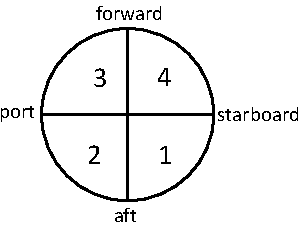
\includegraphics{Fig_trd_quad}
\caption{\label{fi:trd_quad}Transducer divided into four quadrants. The labels are directions often used when a transducer is mounted on a ship.}
\end{figure}
%


\subsection{Power and angle samples}
The transceiver measures voltage over a load, $\zrxe$, connected in series with the transducer impedance, $\ztde$. When calculating various acoustic properties a system gain parameter will be used which assumes a matched receiver load. The total received power, $\prxe(\samplesymt)$, from all transducer sectors for a matched receiver load (Fig. \ref{fi:impedances}) is given by: 
\begin{equation}
\label{eq:prx}
\prxe(\samplesymt) = \nchannels\left( \frac{|\ypc(\samplesymt)|}{2\sqrt{2}} \right)^2 \left( \frac{|\zrxe+\ztde|}{\zrxe} \right)^2 \frac{1}{|\ztde|}.
\end{equation}
%
\begin{figure}
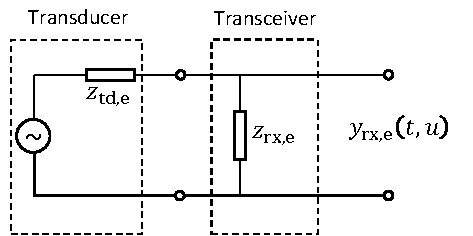
\includegraphics[width=16cm]{Fig_impedances}
\caption{\label{fi:impedances}Equivalent circuit diagram of transducer/transceiver with system impedances.}
\end{figure}

Forward/aft and port/starboard phase angles of target echoes are estimated by combining the transducer half signals thus: 
%
\begin{eqnarray}
\label{eq:phase1}
y_\along(\samplesymt) & = & y_{\textrm{pc,fore}}(\samplesymt) y_{\textrm{pc,aft}}^*(\samplesymt), \\
y_\athw(\samplesymt) & = & y_{\textrm{pc,star}}(\samplesymt) y_{\textrm{pc,port}}^*(\samplesymt),
\end{eqnarray}
%
where $y_\along(\samplesymt)$ is the electrical angle along the minor axis of the transducer (positive in the forward direction when ship-mounted) and $y_\athw(\samplesymt)$ the electrical angle along the major axis of the transducer (positive to starboard when ship-mounted), where complex signals are represented in the form $e^{j 2\pi \freqsym \timesym}$, where $j = \sqrt{-1}$. The physical echo arrival angles ($\along$ and $\athw$) are then given by:
%
\begin{eqnarray}
\label{eq:phase2}
\along(\samplesymt) & = & \arcsin\left( \frac{\atan\left( \Im(y_\along(\samplesymt)), \Re(y_\along(\samplesymt) \right)}{\anglefalong}\right) \\
\athw(\samplesymt) & = & \arcsin\left( \frac{\atan\left( \Im(y_\athw(\samplesymt)), \Re(y_\athw(\samplesymt) \right)}{\anglefathw}\right).
\end{eqnarray}
%
where $\anglefalong$ and $\anglefathw$ are constants that convert from phase angles to physical echo arrival angles and are derived from the transducer geometry and $\fc$ the centre frequency of the chirp pulse \citep{ehrenberg1979}. The inverse sine is indicated by $\arcsin$, the four quadrant inverse tangent which returns values in the interval $[-\pi, \pi]$ inclusive is indicated by $\atan$, the real part of a complex number by $\Re$ and the imaginary part by $\Im$. As a mnemonic, the horizontal line in the symbol used for the forward/aft direction, $\along$, represents the pivot axis for the alongship angles and the near-vertical line in the $\athw$ symbol indicates the pivot axis for port/starboard angles.
%
\begin{figure}
\includegraphics[width=16cm]{Fig_theta_phi}
\caption{\label{fi:theta_phi}Physical angles $\along$ and $\athw$.}
\end{figure}

\section{Target strength}

To illustrate each step of the process to obtain $TS(m)$ we use a single ping from a data file where a single metallic calibration sphere with 35 mm diameter (WC35) is suspended approximately 6 m below a 120 kHz transducer (fig.~\ref{Fig_TS_echogram}). 

\begin{figure}
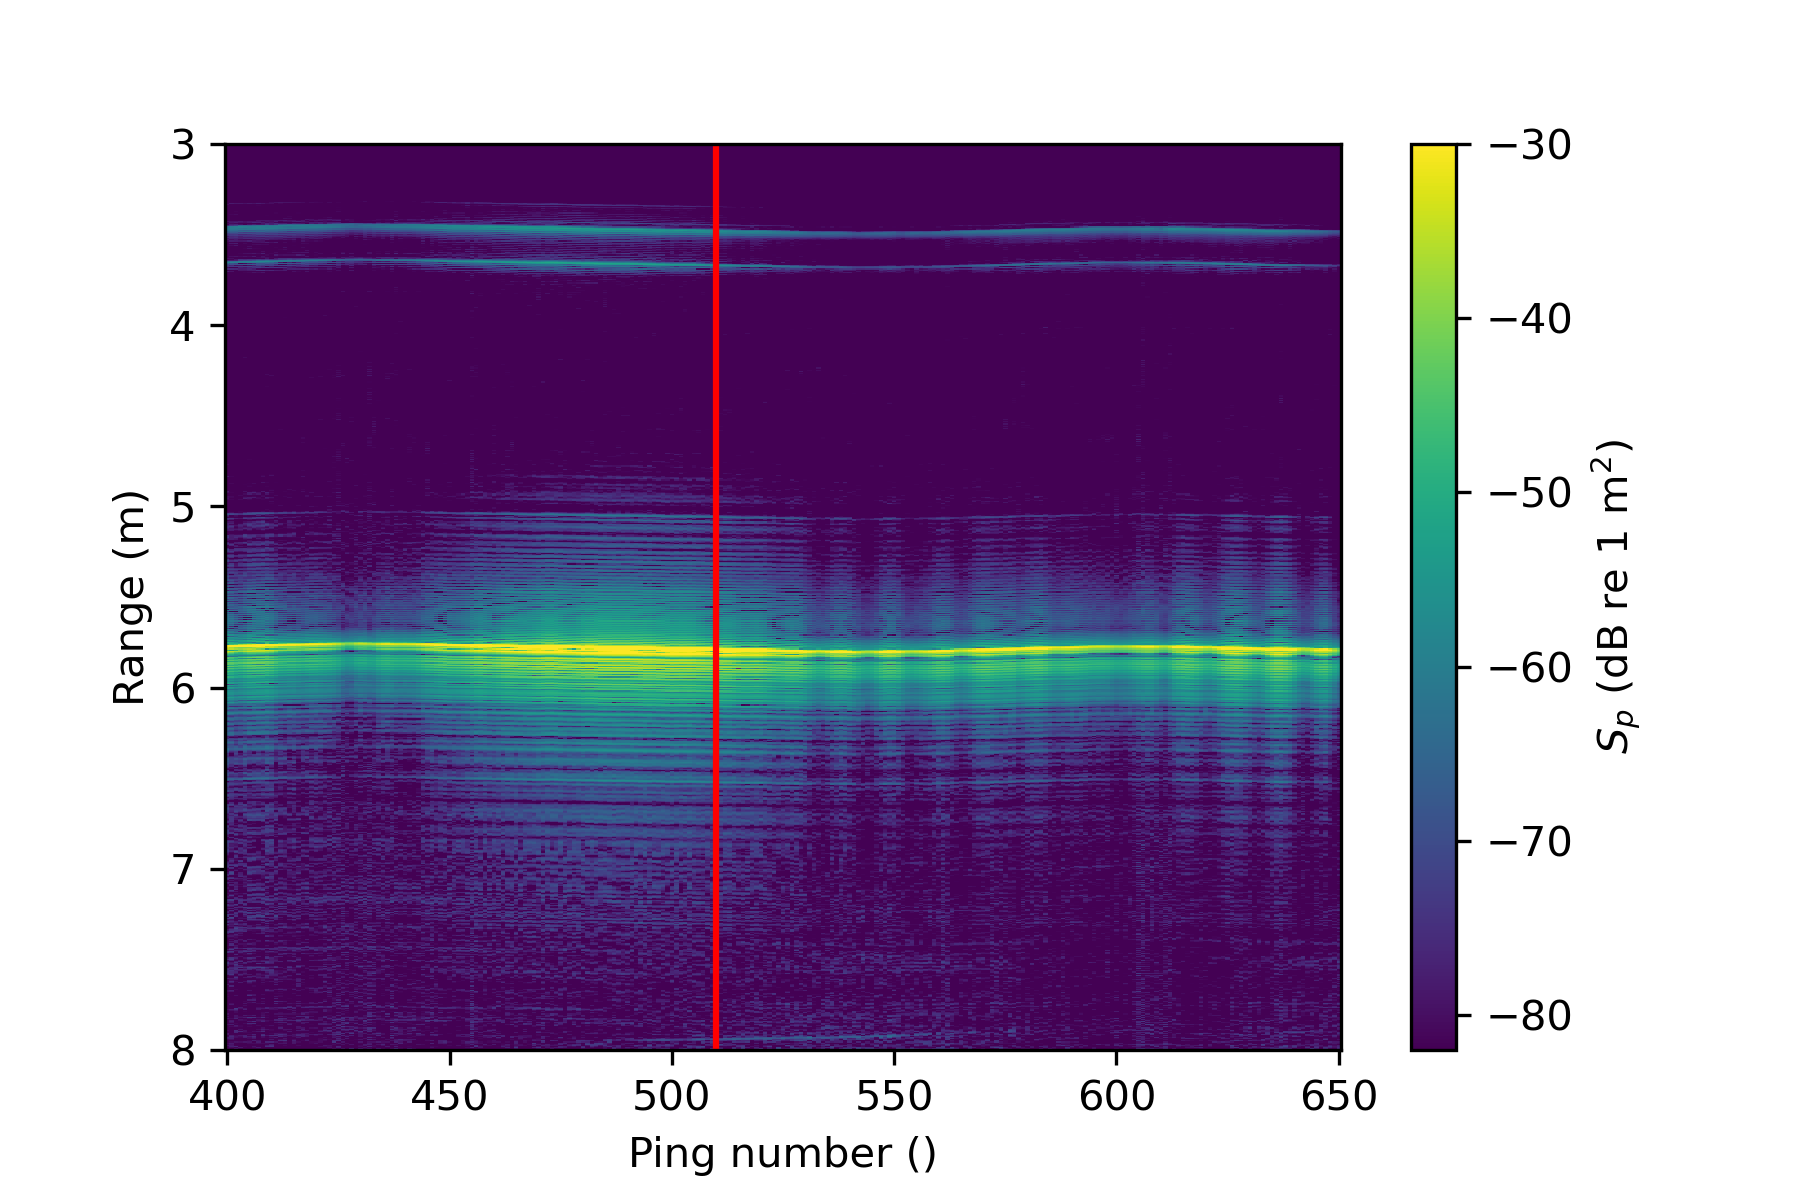
\includegraphics[width=16cm]{Fig_TS_echogram}
\caption{\label{Fig_TS_echogram} Sv as a function of frequency ($m$) and range ($n$) for a echogram raw data file. The red vertical line indicates ping to be processed in this section for TS(m). Single target calibration sphere is seen at approximately 6 m range and the seafloor at approximately 12 m.}
\end{figure}

Echoes from single targets are often characterised by their $\ts$, which is related to the differential backscattering cross section, $\bs$, via
%
\begin{equation}
\label{eq:TS_bs}
\ts = 10\log_{10}\left(\frac{\bs}{\rangeref^2}\right),
\end{equation}
%
where $\log_{10}$ is the logarithm with base 10 and $\rangeref$ is 1 m.

The power-budget equation (i.e., sonar equation) for a single target \citep[Formulation D, ][]{lunde2016} at frequency $\freqsym$ is:
%
\begin{equation}
\label{eq:TS}
\ts(\freqsym) = 10\log_{10}(\prxetf(\freqsym)) + 40\log_{10}(\range) + 2\absorp(\freqsym) \range 
- 10\log_{10}\left( \frac{\ptxe \wlen^2(\freqsym) \gain^2(\along_t,\athw_t,\freqsym)}{16\pi^2} \right),
\end{equation}
%
where $\prxetf(\freqsym)$ is the Fourier transform of the received electric power in a matched load for a signal from a single target at frequency $\freqsym$, $\range_t$ is the range to the target, $\absorp$ the acoustic absorption at frequency $f$, $\ptxe$ the transmitted electric power, $\wlen$ the acoustic wavelength, and $\gain$ the transducer gain incorporating both the on axis gain $\gain_0(\freqsym)=\gain(0,0,\freqsym)$ and the beam pattern based on the estimated target bearing $(\along_t,\athw_t)$.

The point scattering strength, $\mysp(\samplesymt)$, is estimated by applying Eq. \ref{eq:TS} to the received digitized power samples using the on-axis gain value with $f$ set to the centre frequency of the broadband pulse, $\fc$: 
\begin{equation}
\label{eq:Sp}
\mysp(\samplesymt) = 10\log_{10}(\prxe(\samplesymt)) + 40\log_{10}(\range(\samplesymt)) 
+ 2\absorp(\fc) \range(\samplesymt) - 10\log_{10}\left( \frac{\ptxe \wlen^2(\fc) \gainzero^2(\fc)}{16\pi^2} \right),
\end{equation}
%
noting that $\mysp(\samplesymt)$ is an average over frequency of all echoes from single or multiple targets received at sample $\samplesymt$.

Based on the point scattering strength samples and the phase angle samples, single targets can be detected, and range and bearing to the single targets can be estimated. This is typically achieved through a single echo detection algorithm (SED). Here we will assume that the samples from the pulse compressed data $\ypc(\samplesymt)$ originating from single target already have been identified, noting that the number of samples after the detected target may be higher than those those before the peak to include scattering processes for beyond ideal point targets. The alongship angle $\along_n$, athwartship angle $\athw_n$ and range $r_n$ at the \emph{peak} power $\prxe(\samplesymt)$ within the detected target is used as estimates for $\along_t$, $\athw_t$ and $r_t$, respectively (Fig. \ref{fi:TS}. A simple pseudo SED algorithm is implemented in the code for illustrative purposes.

From the autocorrelation function of the matched filter signal, $\ymfauto(\samplesymt)$, the equivalent number of samples around the peak are extracted to create the reduced autocorrelation signal of the matched filter signal, $\ymfautored(\samplesymt)$. Depending on the target scattering characteristics and the distance to any adjacent single targets, the number of samples around the peak echo level in $\ypctarget(\samplesymt)$ that contain the majority of the echo energy can be more or less than the total number of samples around the peak of $\ymfauto(\samplesymt)$. If the number of samples around the target is more than the total number of samples around the peak of $\ymfauto(\samplesymt)$ all samples around the peak of $\ymfauto(\samplesymt)$ are used. If the number of samples around the target is less than the total number of samples around the peak of $\ymfauto(\samplesymt)$, this lower number is used to create a reduced autocorrelation signal, $\ymfautored(\samplesymt)$.
%
\begin{figure}
\includegraphics[width=16cm]{Fig_singleTarget}
\caption{\label{fi:SED} The $\prxe(\samplesymt)$ power (upper) and split beam angles ($\along_t$ and $\athw_t$) (middle) for the single target. The vertical line corresponds to the range $r_t$ for the single target. The $\ymfautored(\samplesymt)$ (lower) is the autocorrelation function of the transmit signal reduced to the length of the target signal and aligned with the peak power of the target.}
\end{figure}

The discrete Fourier transforms of the target signal, $\ypctargetf(\samplesymf)$, and the reduced auto correlation signal, $\ymfautoredf(\samplesymf)$, are given by:
\begin{eqnarray}
\label{eq:DFT_Target_Auto}
\ypctargetf(\samplesymf) & = & \dft_\ndft(\ypctarget(\samplesymt)),\\
\ymfautoredf(\samplesymf) & = & \dft_\ndft(\ymfautored(\samplesymt)),
\end{eqnarray}
where $\dft$ indicates the Fourier transform of length $\ndft$ and $\samplesymf$ the sample index in the frequency domain.
The nomalized discrete Fourier transform of the target signal, $\ypctargetnormf(\samplesymf)$, (Fig. \ref{fi:TS}) is then calculated by: 
%
\begin{equation}
\label{eq:DFT_Target_Auto_Norm}
\ypctargetnormf(\samplesymf) = \frac{\ypctargetf(\samplesymf)} {\ymfautoredf(\samplesymf)}.
\end{equation}
%
\hl{The corresponding frequencies f\_m\_t (?) are calculate as follows... 

See the function EK80CalculationPaper.calcDFTforTS. Nils Olav did not quite get this so please enlighten me...}

Assuming, as a first approximation, that the impedances of the transceiver and transducer are independent of frequency, the received power into a matched load, $\prxetf(\samplesymf)$, is then estimated by:
\begin{equation}
\label{eq:prx_FFT_target}
\prxetf(\samplesymf) = \nchannels\left( \frac{|\ypctargetnormf(\samplesymf)|}{2\sqrt{2}} \right)^2 
\left( \frac{|\zrxe+\ztde|}{|\zrxe|}\right)^2 \frac{1}{|\ztde|}, % All channels (*4), matched load (/2), and effective values (/sqrt(2))
\end{equation}
%
noting that any variation of impedance with frequency will be reflected in the $\gainzero$ obtained from the calibration process.

Target strength can then be estimated using Eq. \ref{eq:TS}, but with $\freqsym$ replaced by the discrete index of frequency, $\samplesymf$:
\begin{equation}
\label{eq:TS_f}
\ts(\samplesymf) = 10\log_{10}(\prxetf(\samplesymf)) + 40\log_{10}(\range_t) + 2\absorp(\samplesymf)\range_t 
- 10\log_{10}\left( \frac{\ptxe \wlen_\samplesymf^2 \gain^2(\along_t,\athw_t,f_\samplesymf)}{16\pi^2} \right).
\end{equation}
%
\begin{figure}
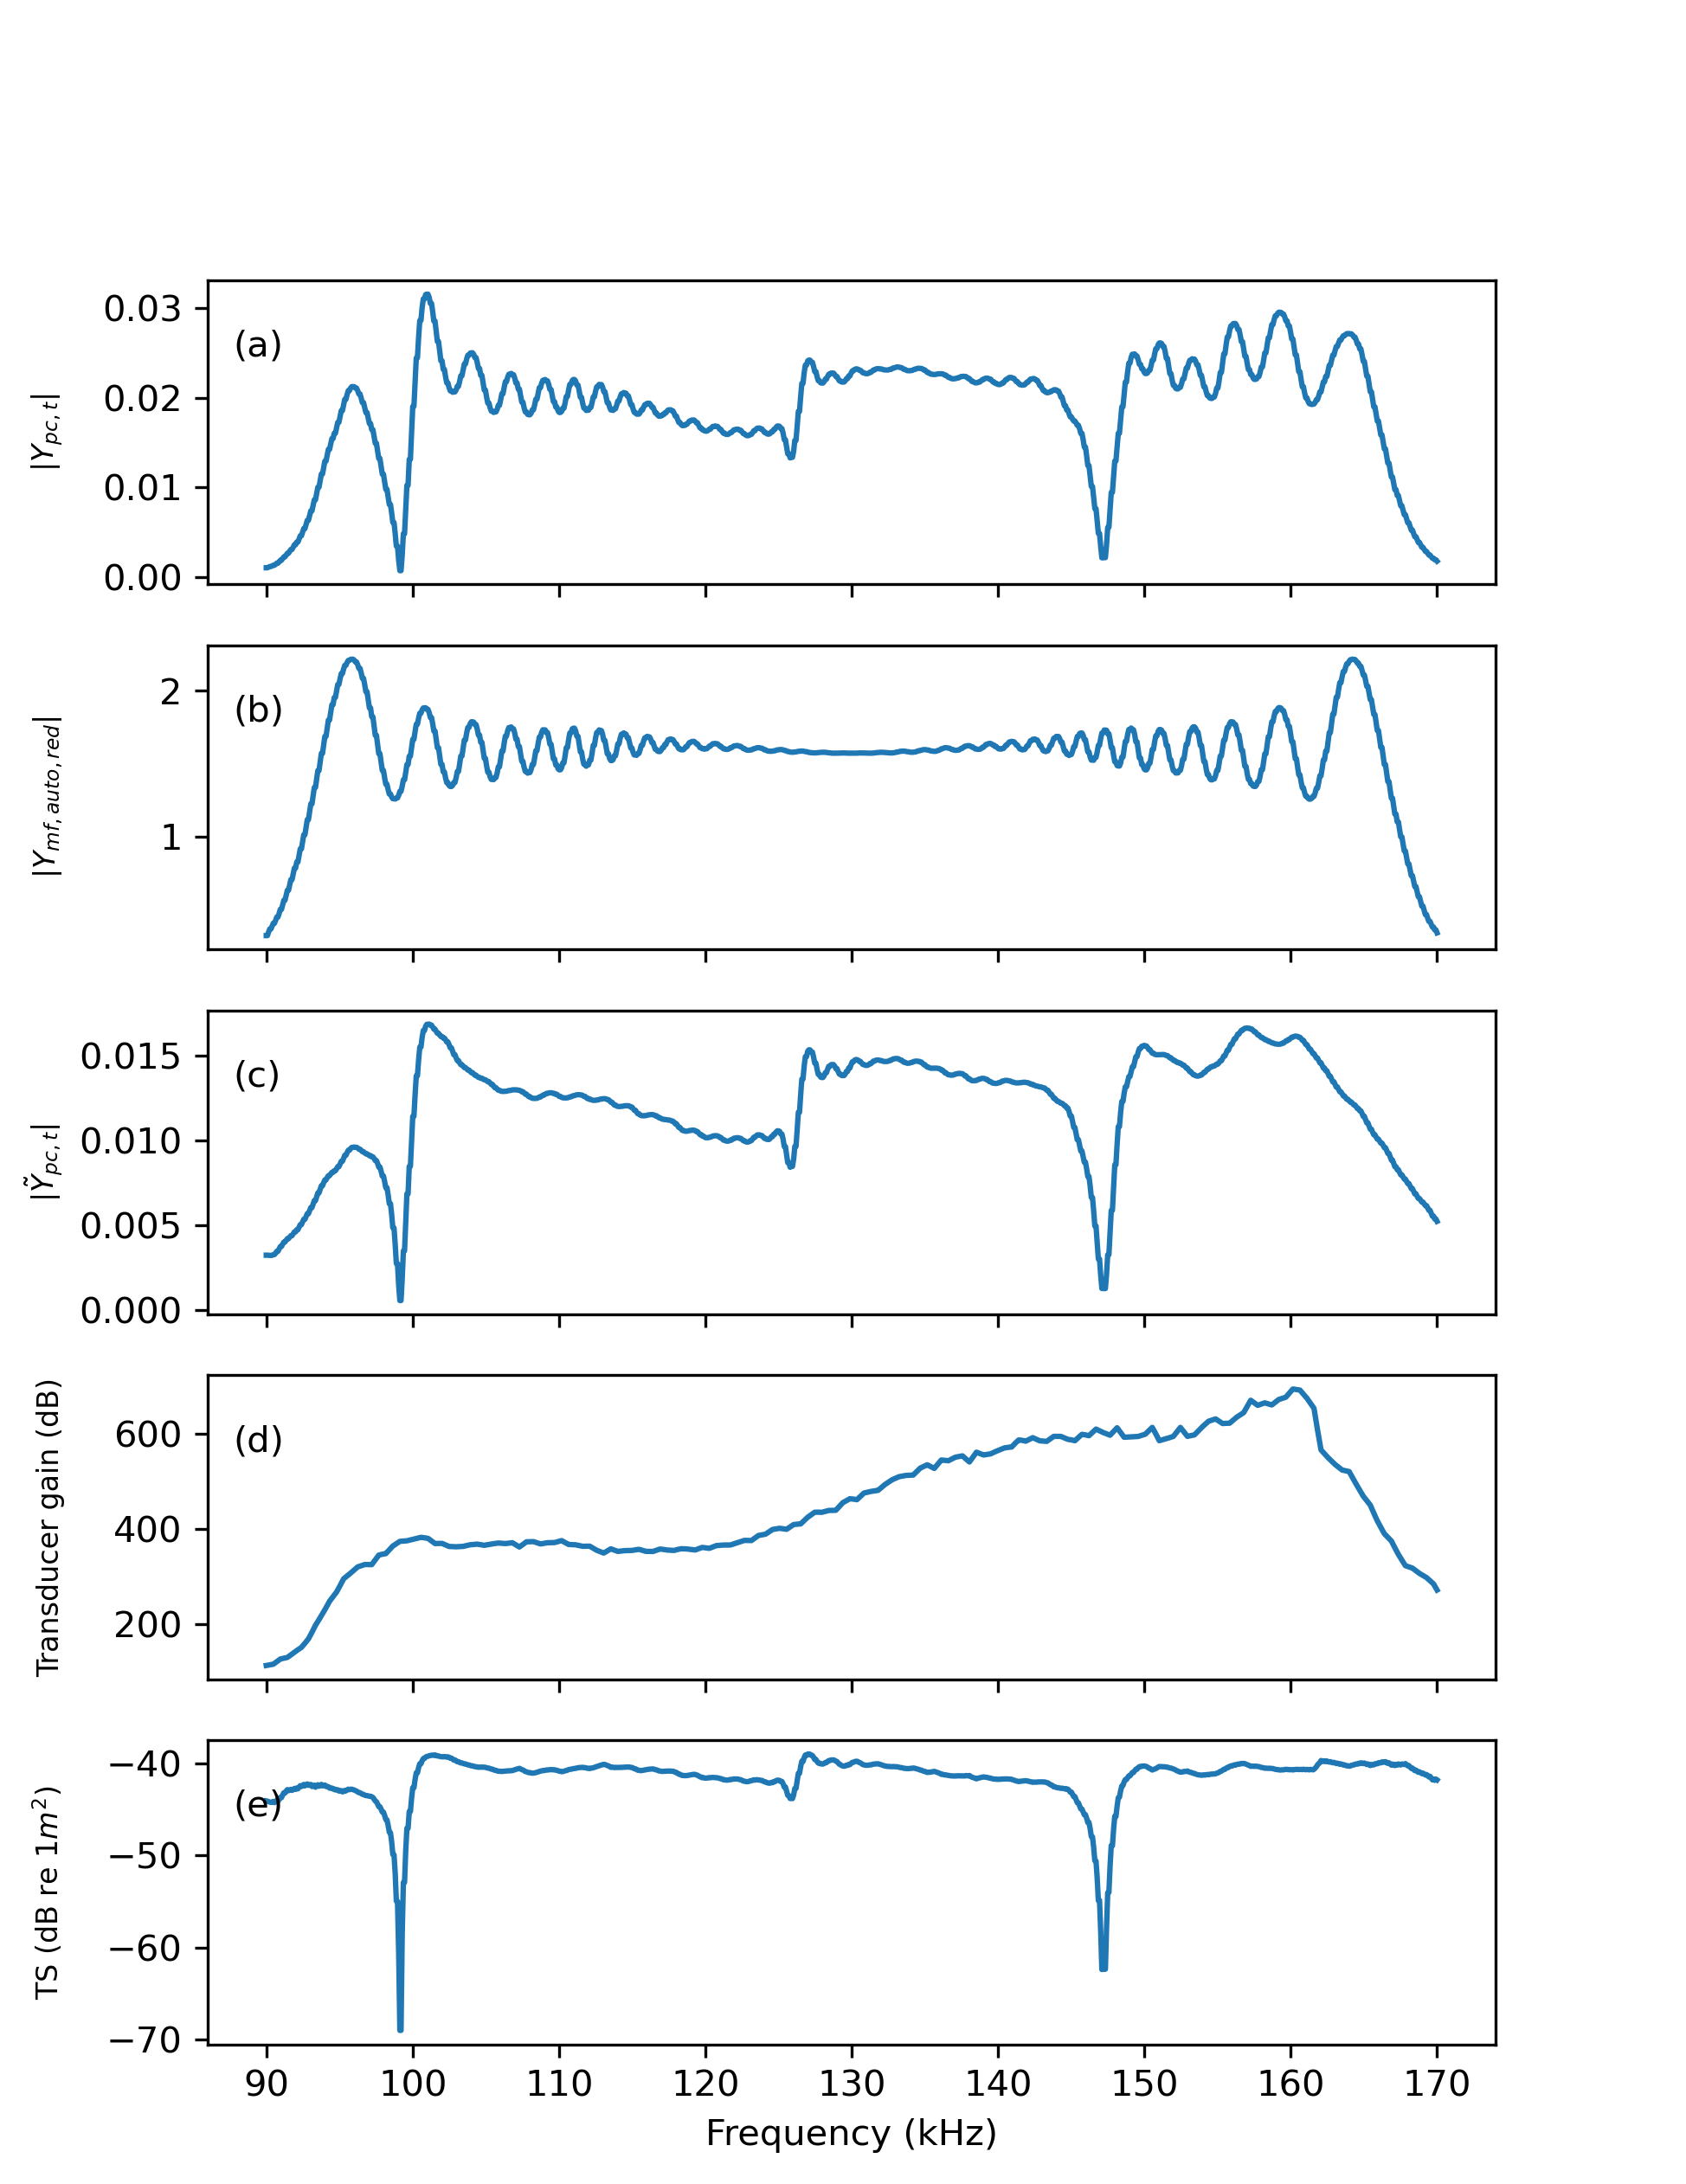
\includegraphics[width=16cm]{Fig_TS}
\caption{\label{fi:TS}The $\ypctargetf(\samplesymf)$ (upper), $\ymfautoredf(\samplesymf)$ (middle) and $\ypctargetnormf(\samplesymf)$ (lower).}
\end{figure}

A frequency modulated pulse scattered by a metallic sphere will exhibit frequencies at which very little energy is returned due to destructive interference \citep{stanton2008}. This is visible in the $\ts$ (Fig. \ref{fi:TS}) and agrees well with theoretical estimates of the backscatter from spheres \citep{maclennan1981}. The amplitude of the backscatter signal also clearly shows these nulls (Fig. \ref{fi:TS}), which are readily visible here due to the use of a linear chirp where time through the pulse corresponds to specific frequencies. 


\hl{Comment from Nils Olav: Using $m$ as an argument to a function is not ideal. If we use the function argument perhaps using $f_m$ would be more logical, i.e. $\lambda(f_m)$. Alternatively using $lambda_m$ is possible. The latter is perhaps more in line with the code since the parameter is an array windexed with $m$ and not a function. $Psi(f)$, on the the other hand is derived from a function, see below.}

\section{Volume backscattering strength}

As a metallic sphere is a rather simple and ideal scatterer, we use $\sv$ from a school of non-swimbladdered fish (\textit{tobis}) (fig.~\ref{Fig_Sv_echogram}) collected with a 120 kHz centre frequency transducer to illustrate the processes to obtain $S_v(m)$. 

Echoes from multiple scatterers can be quantified using volume backscattering strength, $\sv$, being the density of backscattering cross sections, and is given by:
%
\begin{equation}
\label{eq:sv}
\sv  =  10\log_{10}\frac{\sum\bs}{V}.
\end{equation}
%
where $V$ is the volume occupied by the scattering targets. The power-budget equation for multiple targets is then:
%
\begin{equation}
\label{eq:sv_f}
\sv(\freqsym) = 10\log_{10}(\prxevf(\freqsym)) + 20\log_{10}(\range_c) + 2\absorp(\freqsym)\range_c 
- 10\log_{10}\left( \frac{\ptxe \wlen^2 \cw \tslide \eqang(\freqsym) \gainzero^2(\freqsym)}{32\pi^2} \right), 
\end{equation}
%
where $\prxevf(\freqsym)$ is the received electric power in a matched load for the signal from a volume at frequency $\freqsym$, $\cw$ the sound speed, $\tslide$ the duration of the time window, excluding the zero-padded portion if applied, used for evaluating the frequency spectrum, $\range_c$ is the range to the centre of the range volume covered by $\tslide$, and $\eqang$ is the two-way equivalent beam angle. The two-way equivalent beam angle is a function of frequency that is derived from an empirical estimate of $\eqang$ at the nominal frequency, $\fn$:
\begin{equation}
\label{eq:PsiFc}
\eqang(f) = \eqang(\fn)\left(\frac{\fn}{f}\right)^2.
\end{equation}

\begin{figure}
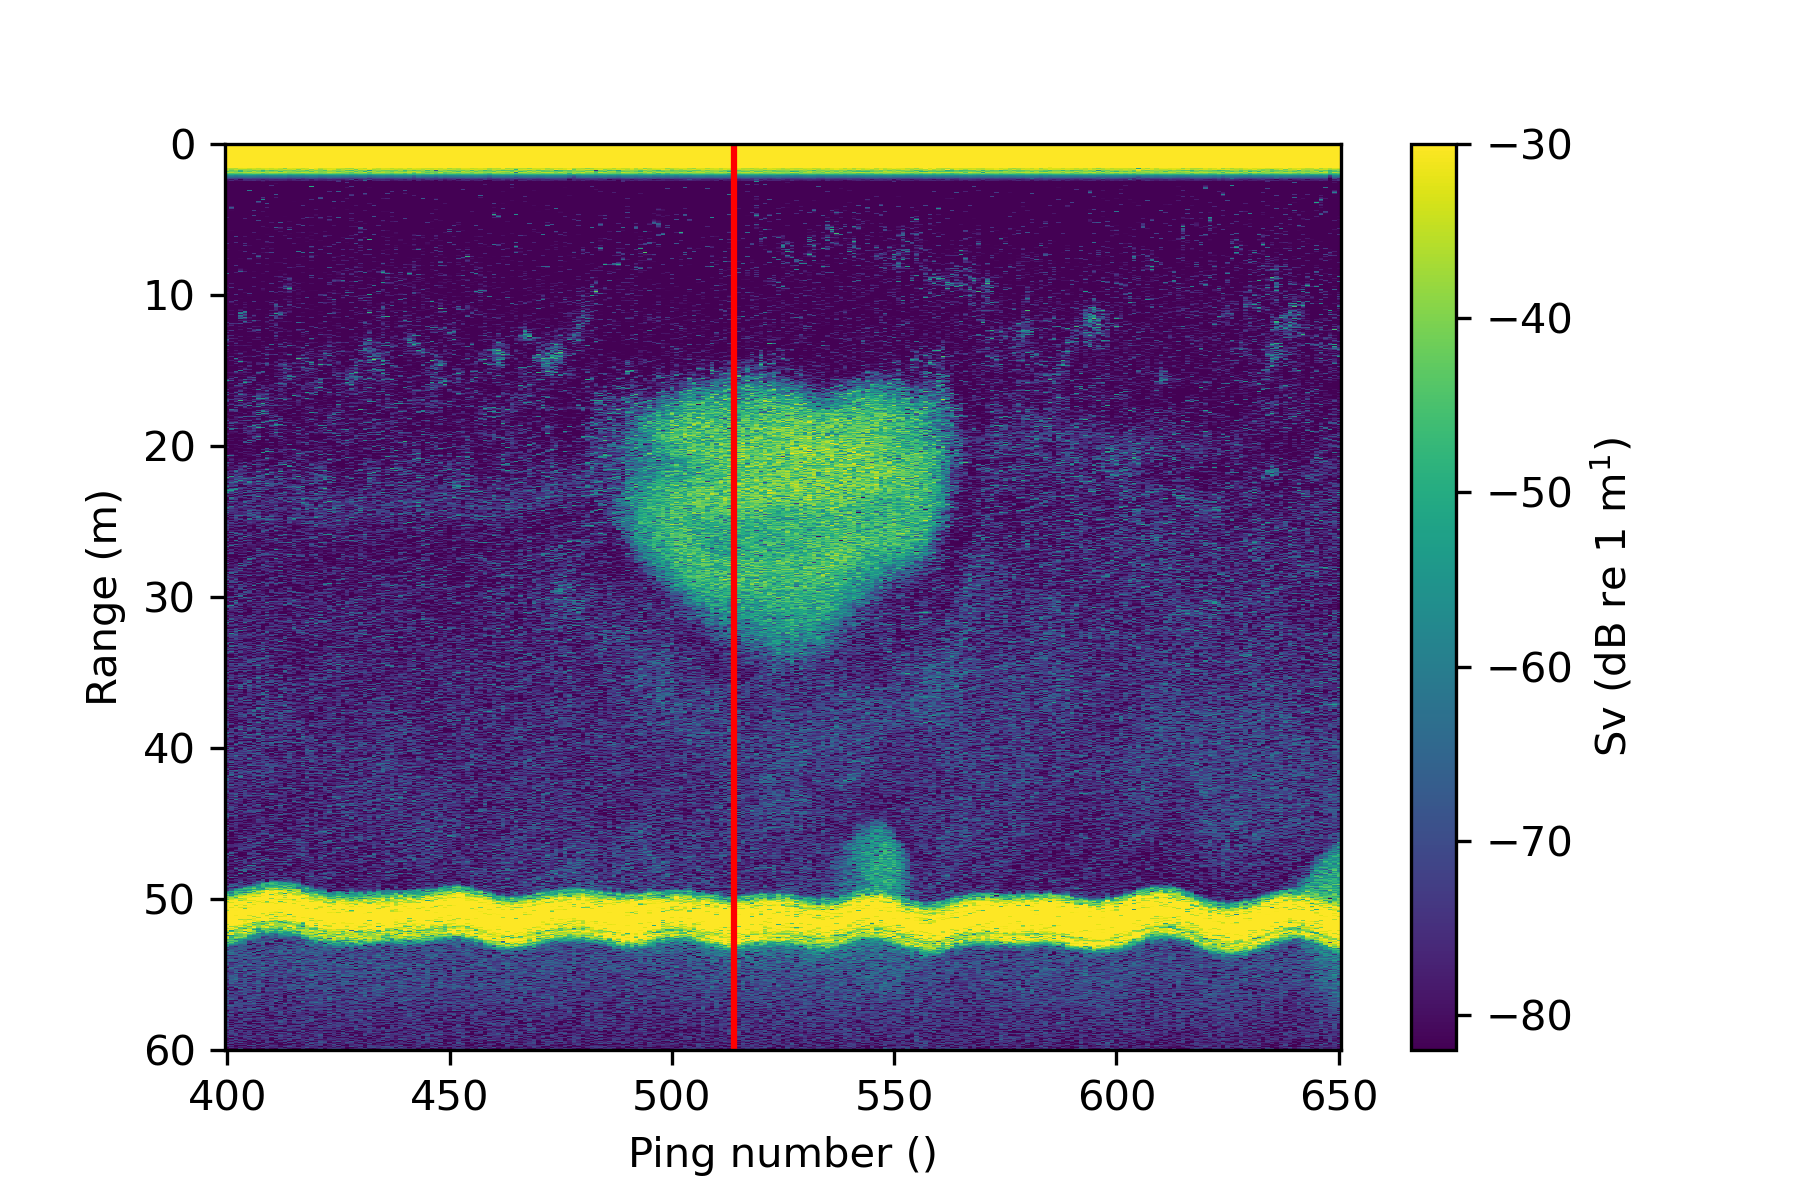
\includegraphics[width=16cm]{Fig_Sv_echogram}
\caption{\label{Fig_Sv_echogram} Sv as a function of frequency ($m$) and range ($n$) for a echogram raw data file. The red vertical line indicates ping to be processed in this section.}
\end{figure}

Volume backscattering samples compressed over the operational frequency band are estimated by applying Eq. \ref{eq:sv_f} to the received digitized power samples using the on-axis gain value with $f$ set to the centre frequency of the broadband pulse, $\fc$:
\begin{equation}
\label{eq:Sv}
\begin{split}
\sv(\samplesymt)  =  10\log_{10}(\prxe(\samplesymt)) + 20\log_{10}(\range_c(\samplesymt)) + 2\absorp(\fc)\range_c(\samplesymt) \\
- 10\log_{10}\left( \frac{\ptxe \wlen^2(\fc) \cw \teff \eqang(\fc) \gainzero^2(\fc)}{32\pi^2} \right),
\end{split}
\end{equation}
noting that $\sv(\samplesymt)$ is an average over frequency of all echoes received at sample $\samplesymt$. In this case, the time window, $\tslide$, is the effective pulse duration, $\teff$, resulting from pulse compression.

Compensation of spherical spreading loss requires compensation of received power by a factor of $r_c^2$, and hence compensation of amplitude by a factor of $\range_c$:
%
\begin{equation}
\label{eq:spreadcomp}
\ypcspread(\samplesymt) = \ypc(\samplesymt)\range_c(\samplesymt).
\end{equation}
%
where $\ypcspread(\samplesymt)$ is the pulse compressed signal compensated for spherical spreading. A discrete Fourier transform is performed on the range compensated pulse compressed sample data using a normalized sliding Hann window, $\hannw(\genidxsym)$. The duration, $\tslide$, of the sliding window is chosen as a compromise between along-beam range resolution and frequency resolution. We suggest that it be at least twice the pulse duration and for computational efficiency reasons should result in a number of samples, $\nw$, which is a power of 2.

\hl{TODO: Explain edge cases.}

The normalised Hann window, $\hannwnorm$, is given by: 
%
\begin{equation}
\label{eq:hannw}
\hannwnorm(\genidxsym) = \frac{\hannw(\genidxsym)}{\left( \frac{||\hannw||_2}{\sqrt{\nw}} \right)}, i = \frac{-\nw}{2}, \ldots, \frac{\nw}{2}
\end{equation}
%
and the discrete Fourier transform of the windowed data, $\ypcvolumef(\samplesymf)$, is then obtained from:
%
\begin{equation}
\label{eq:FFT_volume}
\ypcvolumef(\samplesymf) = \dft_\ndft 
\left( \hannwnorm(\genidxsym) \left(\ypcspread (\genidxsym+\samplesymt) \left[ u(\genidxsym + \frac{\nw}{2}) - u(\genidxsym - \frac{\nw}{2}) \right] \right) \right),
\end{equation}
%
where $u(\genidxsym)$ is the step function and $\samplesymt$ is the sample data index for the centre of the sliding window. The discrete Fourier transform of the auto correlation function of the matched filter signal, $\ymfautof(\samplesymf)$, also needs to be evaluated at the same frequencies:
%
\begin{equation}
\label{eq:FFT_TX_Auto}
\ymfautof(\samplesymf)  =  \dft_\ndft (\ymfauto(\samplesymt)).
\end{equation}

%
\hl{TODO: How to index samples along range? In the code \_n is used to indicate the range component of the FFt's. Needs attention.}

The normalized discrete Fourier transform of the windowed data, $\ypcvolumenormf(\samplesymf)$, is then given by:
%
\begin{equation}
\label{eq:FFT_volume_norm}
\ypcvolumenormf(\samplesymf) = \frac{\ypcvolumef(\samplesymf)}{\ymfautof(\samplesymf)},
\end{equation}
%
and received power into a matched load, $\prxevf(\samplesymf)$, is estimated from:
%
\begin{equation}
\label{eq:prx_FFT_volume}
\prxevf(\samplesymf) = \nchannels \left( \frac{|\ypcvolumenormf(\samplesymf)|}{2\sqrt{2}} \right)^2 \left( \frac{|\zrxe+\ztde|}{|\zrxe|}\right)^2 \\
\frac{1}{|\ztde|}. % All channels (*4), matched load (/2), and effective values (/sqrt(2))
\end{equation}
%
Finally, the discretized estimate of $\sv(\freqsym)$, $\sv(\samplesymf)$, is given by:
%
\begin{equation}
\label{eq:Sv_FFT}
\sv(\samplesymf) = 10\log_{10}(\prxevf(\samplesymf)) + 2\absorp(\samplesymf) \range_c \\
- 10\log_{10}\left( \frac{\ptxe \wlen^2(\samplesymf) \cw \tslide \eqang(\samplesymf) \gainzero^2(\samplesymf) }{32\pi^2} \right).
\end{equation}

By selecting a set of centre samples $n$, $Sv$ values can be presented as a function of range ($n$) and frequency ($m$) for each ping. The range for centre samples $n$ could be chosen to half the window length or any other grid that the user prefer the data presented to be in. This can be useful when combining the $Sv(m)$ across a range of transducers. In our example we have simply chosen n to be on the same order of the range resolution (fig.~\ref{Fig_Sv_m_n}).

\begin{figure}
\includegraphics[width=16cm]{Fig_Sv_m_n}
\caption{\label{Fig_Sv_m_n} Sv as a function of frequency ($m$) and range ($n$) for a single ping}
\end{figure}

For acoustic abundance estimation and classification purposes it is common to integrate the Sv over a range, in our example we integrate $Sv$ from 15 to 34 m covering a school of non-swimbladdered fish (fig.~\ref{Fig_Sv_echogram}). We note that we normally require averaging over several pings to obtain an unbiased estimate of $Sv$ for echo integration purposes. Here we present the $Sv(m)$ over the layer for our example ping for illustrative purposes (fig.~\ref{Fig_Sv_avg}). Even though this is for a single ping, we still observe a positive slope of the frequency response indicative of non-swimbladdered fish. 

\begin{figure}
\includegraphics[width=16cm]{Fig_Sv_avg}
\caption{\label{Fig_Sv_avg} $Sv$ as a function of frequency ($m$) averaged over a range interval covering a fish school }
\end{figure}

The trend for increasing $\sv$ with frequency is well-known \citep{korneliussen2010} and is consistent with the trend observed in this example. In contrast to data from isolated scatterers, such as metallic spheres, the benefit of pulse compression on the backscatter from an object that generates many overlapping echoes is not immediately obvious (fig.~\ref{Fig_Sv_echogram}).

\section{Discussion}

The use of broadband signals in fisheries acoustics is a developing field, and our contribution represents a comprehensive description of data processing steps. The inclusion of a corresponding code ensures a complete description. One could also envision that signal processing steps designed for specific purposes beyond these standard parameters can be developed, and our code may then serve as a starting point for further development. We also envision that the paper and code will be used both for educational purposes and for understanding the standard signal processing.

Choices

The contribution includes all the minor details required for the processing steps to work in practice. This includes steps well founded in the literature as well as practical and more ad-hoc choices, and a few examples of such choices follows. How to handle gaps in the calibration data, the choice of transmit pulse including tapering, calculation of efficient pulse duration, and decimation factors and filtering are examples of such choices. When convolving the received signal with the transmit pulse, there are various approaches to handle edge cases, and, in our implementation, we simply chose to remove the edge cases. We have also assumed a four-sector transducer, and the code must be adapted to other beam configurations if other configurations are needed. The signal processing also assumes a matched load impedance for the transducer and transceiver. Our objective is not to provide an evaluation of these choices, but to serve as a reference implementation when benchmarking the choices.

$\ts(\freqsym)$ is a common metric for studying single targets, used to extract features for single individuals. These features includes size, target classification and is used to extract behaviour through tracking. In our implementation, the target strength by frequency calculation assumes that a single target has successfully been identified. For this to work in proactive a robust single target detector is required. Several single echo detection algorithms exist, and various single echo detection algorithms may be required depending on situation. Typical SED algorithms are based on traditional single frequency pulses, and utilizing the information in the broadband data improved SEDs may be envisioned, but this is outside the scope of this paper.

$\sv(\freqsym)$ is a key parameter for echo integration. To estimate $\sv(\freqsym)$ a Fourier transform is used, repeatedly applied via a sliding window in range. The recommended size of the window is two times the pulse length, and is chosen as a compromise between spatial and frequency resolution. Since the duration of the sliding window can cause the spreading loss compensation to differ between the beginning and end of the window, the compensation for spreading loss is performed on the pulse compressed time domain data before the transform. Absorption loss compensation is also range dependent (and frequency dependent), but is insignificant for typical operating frequencies at short ranges and between the beginning and the end of the window at longer ranges. The compensation for absorption loss is therefore performed after applying the discrete Fourier transform. The choice of window also allow the data to be cast on a predefined range-frequency grid, which can be used to fit data across transducers to an n-dimensional tensor typically employed by machine learning frameworks like Keras, Pytorch, and Tensor flow.

The formulation presented in this paper results in several frequency dependent parameters, such as transducer gain, two-way equivalent beam angle, and the water absorption coefficient, that are required to quantitatively estimate $\ts(\freqsym)$ and $\sv(\freqsym)$ from received broadband signals. Methods to estimate these are not within the scope of this paper, but common practise is to use the conventional sphere backscatter calibration methodology \citep{demerCalibrationAcousticInstruments2015} slightly enhanced for broadband \citep{hobaekCharacterizationTargetSpheres2013,lavery2017}. We note that these methods do not provide an operational method to estimate $\teff$ or $\Phi(f)$, especially for ship-mounted transducers, and that empirical measurements of these parameters are necessary to fully calibrate both narrowband and broadband echosounders.

A set of equations for calculating calibrated, frequency-dependent, target strength and volume backscatter from broadband echosounder signals have been presented. Providing an open-source resource for anyone interested in learning and developing the techniques further.  

Old Discussion below

The use of broadband signals in fisheries acoustics is a developing area and we anticipate many valuable enhancements will occur in the coming years. For example, the use of $\ts(\freqsym)$ and $\sv(\freqsym)$ to improve acoustic target classification \citep{bassett_broadband_2018, korneliussen2018}, and the potential of the high range resolution from pulse compression to observe small-scale fish behviours \citep{skaret_diel_2020} and to detect objects adjacent to boundaries \citep{lavery2017}. The basic formulation for calculating $\ts(\freqsym)$ and $\sv(\freqsym)$ presented here provides the foundation for future enhancements.

In this implementation (ref code) several choices have been made. Some of these are well founded in signal processing literature whereas others are of a more practical and ad-hoc nature, where other approaches could been equally valid. These include, as examples,
\begin{itemize}
\item How to handle calibration, interpolation, missing calibration
\item Transmit pulse
\item Tapering of the transmit pulse
\item Decimation factors and filters
\item When Convoling the recieved signal with the transmit pulse - edge cases
\item Assuemd four sector transducer
\item Matched load - hvor stor effekt å gå utover 
\item Assumed an impedance (trancuder)
\item Effective pulse duration...
\item Assuming SED algorithm, know the target depth. Improvements possible (SED for broadband). Number of samples for pulse comp - what is included, dense aggregations, sidelobes - pc, ...
\item Window size
\item Edge cases - removed
\end{itemize}

To estimate $\sv$ as a function of frequency a Fourier transform is used, repeatedly applied via a sliding window in range. However, the duration of this sliding window can be so long that the difference in spherical spreading loss compensation ($r_c^2$, implemented as the $20\log_{10}(\range_c)$ term in Eq. \ref{eq:Sv}) from the beginning of the window to the end can be significant, particularly for short range measurements. Thus, compensation for spreading loss is performed before applying the discrete Fourier transform. Absorption loss compensation is also range dependent (and frequency dependent), but since absorption loss compensation is insignificant for typical operating frequencies at short ranges and the difference in absorption loss compensation between the beginning and the end of the sliding window is insignificant at longer ranges, compensation for absorption loss is performed after applying the discrete Fourier transform.

...

Modern machine learning techniques are well suited for further processing of broadband echosounder data. Deep learning algorithms, including deep clustering, provide powerful methods to tease out patterns from high dimensional and complex data. By providing similar step sizes across frequencies it is possible to adapt this code to for an n-dimensional tensor typically employed by machine learning frameworks like Keras, Pytorch, and Tensor flow. 

The formulation presented in this paper results in several frequency dependent parameters, such as transducer gain, two-way equivalent beam angle, and the water absorption coefficient, that are required to quantitatively estimate $\ts(\freqsym)$ and $\sv(\freqsym)$ from received broadband signals. Methods to estimate these are not within the scope of this paper, but common practise is to use the conventional sphere backscatter calibration methodology \citep{demerCalibrationAcousticInstruments2015} slightly enhanced for broadband \citep{hobaekCharacterizationTargetSpheres2013, lavery2017}. We note that these methods do not provide an operational method to estimate $\teff$ or $\eqang(\freqsym)$, especially for ship-mounted transducers, and that empirical measurements of these parameters are necessary to fully calibrate both narrowband and broadband echosounders.

The processing equations and methodology presented in this paper have been implemented in version 1.12.4 and earlier of the \ek{} software.

\section{Conclusion}

A set of equations for calculating calibrated, frequency-dependent, target strength and volume backscatter from broadband echosounder signals have been presented, with reference to the \ek{} echosounder.

\section{Data Availability Statement}

The data associated with this article are available on request from the authors.

\bibliography{Reference_database}


\end{document}
